In the real world pinhole cameras aren't practical because, if the pinhole is large the image is blurred and if it's small the image is dim. For this reason we use lenses which refocus incoming rays onto the image plane. Because of the use of lenses, distortion occurs. Here we will go over radial and tangential distortion. \\
Let $(x, y)$ be the coordinates of a point on the undistorted image and $(x_d, y_d)$ the coordinates of that same point on the distorted image. \\

Radial distortion the "barrel" or "fish-eye" effect that occurs in images. We can represent radial distortion as
\begin{gather}
    x_d = x(1 + k_1 r^2 + k_2 r^4 + k_3 r^6) \notag\\
    y_d = y(1 + k_1 r^2 + k_2 r^4 + k_3 r^6) \notag\\
    r^2 = x^2+y^2
    \label{radialdistEq}
\end{gather}

\begin{figure}[h]
    \centering
    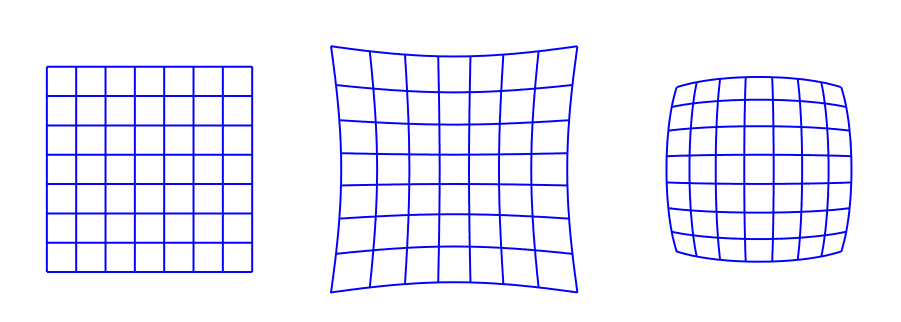
\includegraphics[width=0.5\linewidth]{imgs/radialdist.png}
    \caption{Radial distortion}
    \label{fig:raddist}
\end{figure}

Tangential distortion occurs because the lenses are not perfectly parallel to the imaging plane and it can be represented as

\begin{gather}
    x_d = x+[2p_1xy+p_2(r^2+2x^2)] \notag\\
    y_d = y+[p_1(r^2+2y^2)+2p_2xy]
    \label{tangentialdistEq}
\end{gather}

To find out the distortion coefficients $(k_1, k_2, p_1, p_2, p_3)$ and the intrinsic and extrinsic parameters we perform camera calibration. 